
\subsection{The Hui Problem}\label{ss:hui}

The Implosion problem described in Section 4.7 of  Liska and Wendroff \cite{Liska} was first used by Hui, Li, and Li \cite{Hui} and also, with variants, by Chang, Wang, and Chow \cite{Chang} as a two-dimensional test problem for the Euler equations.  The geometry of the problem is shown in Figure \ref{fig:HuiGeom} where a square box is filled with a gas having $\gamma = 7/5$ and has a diaphragm along the line from point $a$ to point $b$, both of which are a distance $h$ from the origin as shown.  In the cases presented here, $S = 0.3$, $h = 0.15$ with either $\beta = 0 \ \mathrm{rad.}$ or $0.4\ \mathrm{rad.}$  The mesh is rotated as a check of the independance of mesh orientation on the results in Flexi.  In \ref{ssec:hoprin-hui-Rot0} the ``hopr'' mesh input file for the $400 \times 400 \times 1$ element unrotated hexahedral mesh is given while that for the rotated mesh is in \ref{ssec:hoprin-hui-Rot}.

\begin{figure}[h!]
 \begin{center}
  \input{figures/HuiGeometry.pdf_t}
  \caption{The two-dimensional Hui implosion problem geometry.  Points $a$ and $b$ lie on the sides of a square box each a distance $h$ from the origin. The box sides are $S$ in length and is rotated about the origin by an angle $\beta = \frac{\pi}{2} - \alpha$. The line $\overline{ab} = [\sin(\beta) - \cos(\beta)] y - [\sin(\beta) + \cos(\beta)] x + h = 0$.}
  \label{fig:HuiGeom}
 \end{center}
\end{figure}

\subsubsection{Non-rotated Mesh Results}\label{sssec:huiNR}

In \ref{ssec:flexiin-hui-Rot0} the Flexi input data file is given for the unrotated mesh.  It is noted that in those files, the $\mathrm{IniExactFunc}  = 1346$ value was added to the exactfunc.f90 source code so that the Hui problem initial conditions could be applied to the mesh using the additional input variable: $\mathrm{Hui\_Data} = (/\beta, h/)$ (rotation angle in radians, interface distance along box side).  If $X(1) + X(2) > h$, then use $\mathrm{RefState} = (1.0, 0., 0., 0.,  1. )$ (density, x vel, y vel, z vel, pressure), otherwise use $\mathrm{RefState} = (0.125, 0., 0., 0., 0.14 )$ in the low energy region. In addition, the new variable $\mathrm{IndSym} = 1$ is used to switch on a modification to the Persson indicator (in flexi/src/indicator/indicator.f90) assuring that it is symmetric for this problem.

Results for the Hui problem are shown in Fgure~\ref{fig:hui-Rot0} for the initial state (Fig. \ref{fig:hui-Rot0-0}) as well as for $t = 0.05$ and $t = 2.5$.  The early time results (Fig.~\ref{fig:hui-Rot0-005}) compare favorably with Fig.\ 4.10 (especially for WENO and CLAW methods) of Liska and Wendroff \cite{Liska}.  The late time results in Fig.~\ref{fig:hui-Rot0-250} compare favorably with the results of Liska and Wendroff in their Fig.\ 4.11.  That reference (\cite{Liska}) also has links to various animations which are very informative.

\begin{figure}[h!]
\centering
\begin{subfigure}[h!]{0.4\linewidth}
\centering
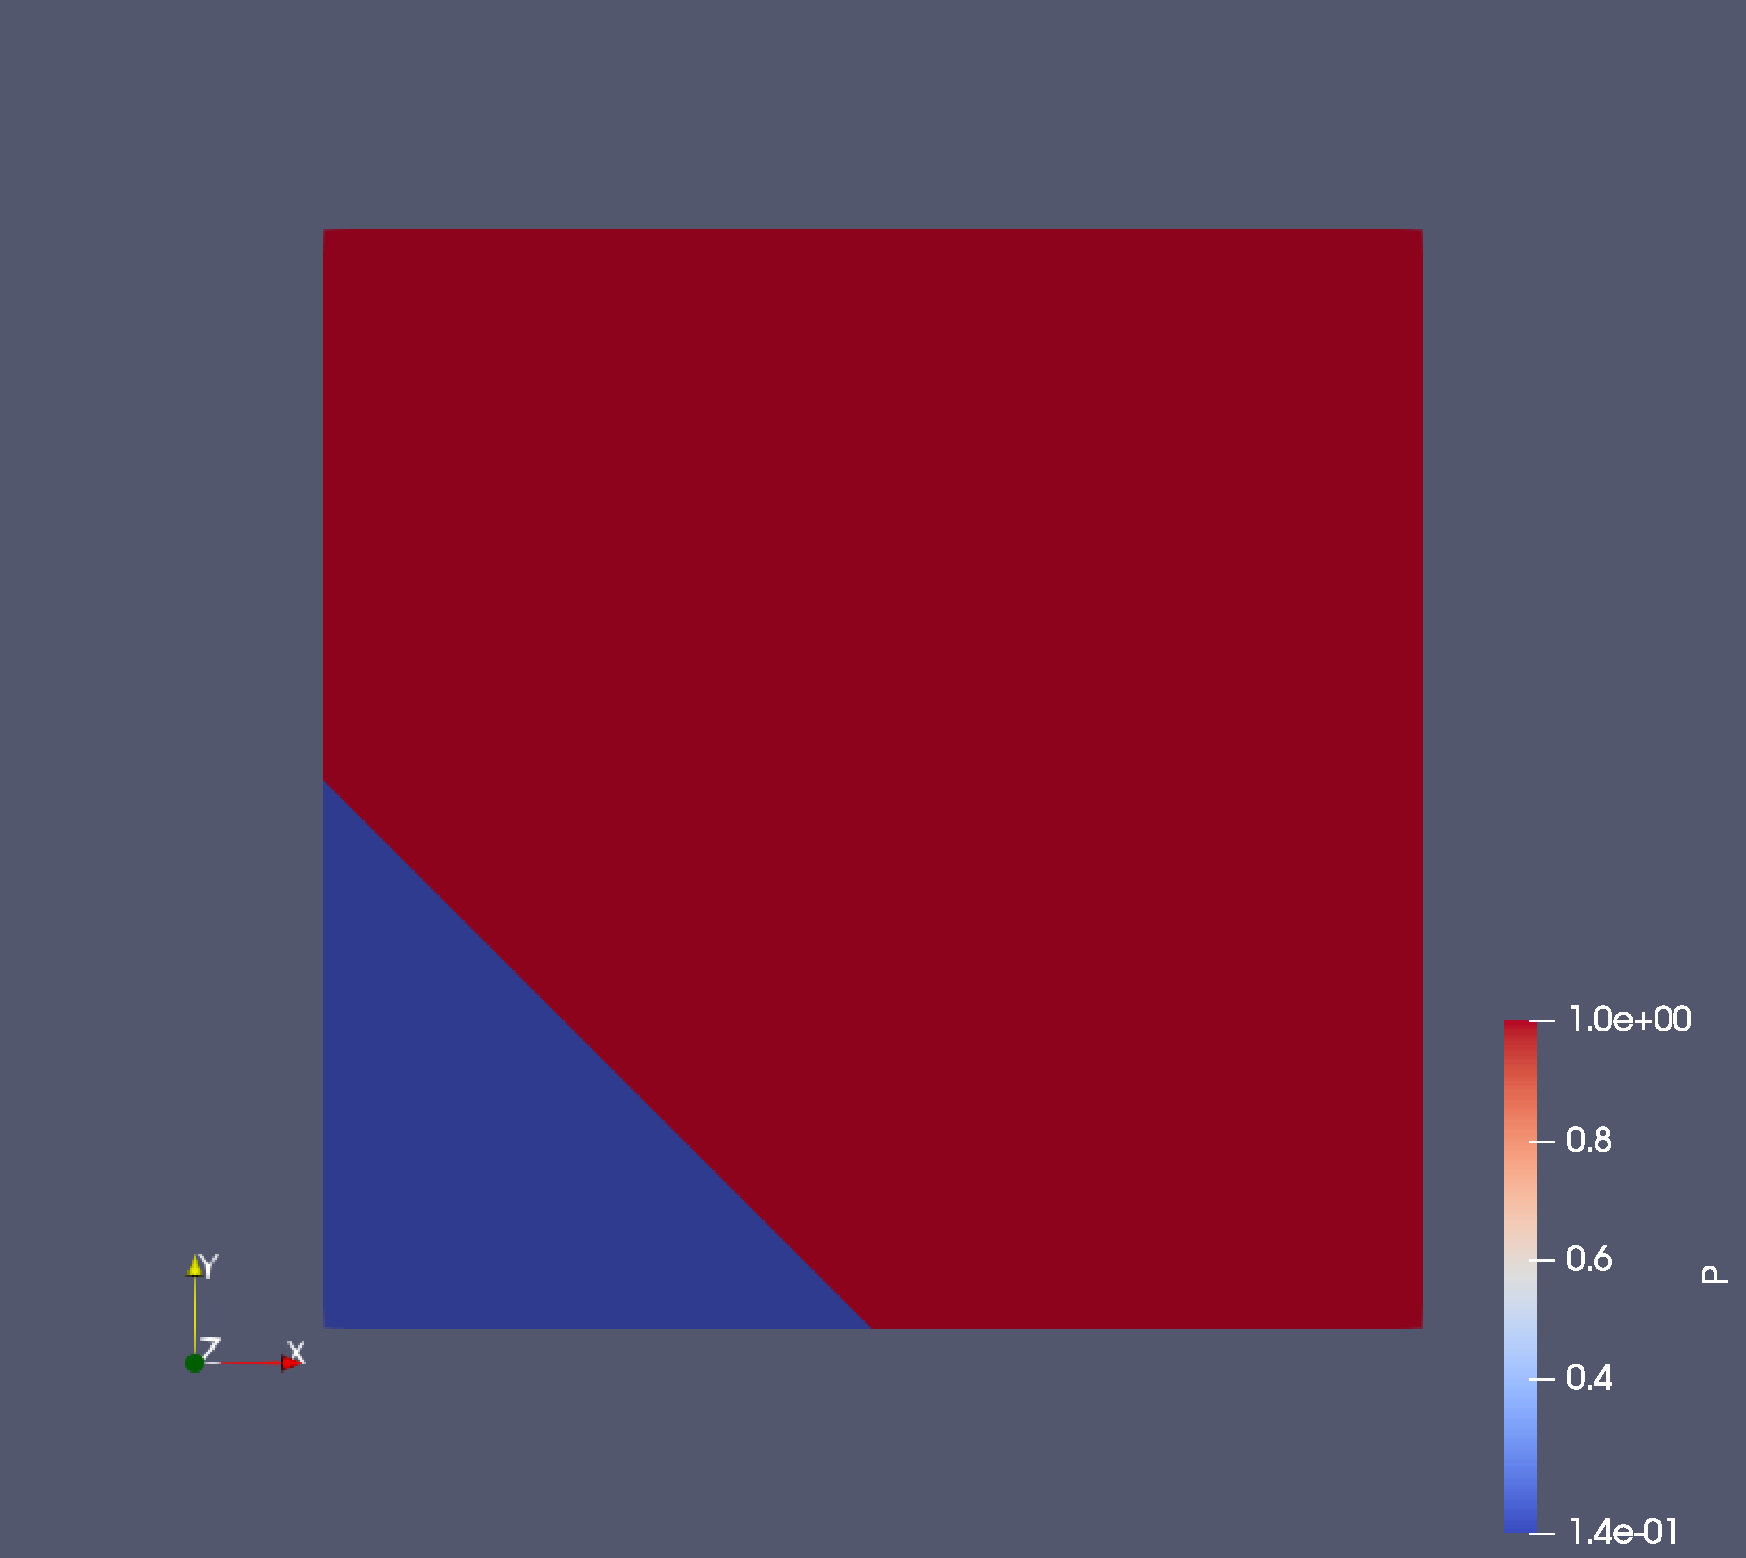
\includegraphics[scale=0.16]{figures/GAH-Hui-400-000.pdf }
\caption{Initial pressure field for the $\beta = 0.$ Hui problem.\bigskip \bigskip}
  \label{fig:hui-Rot0-0}
\end{subfigure}
\begin{subfigure}[h!]{0.4\linewidth}
\centering
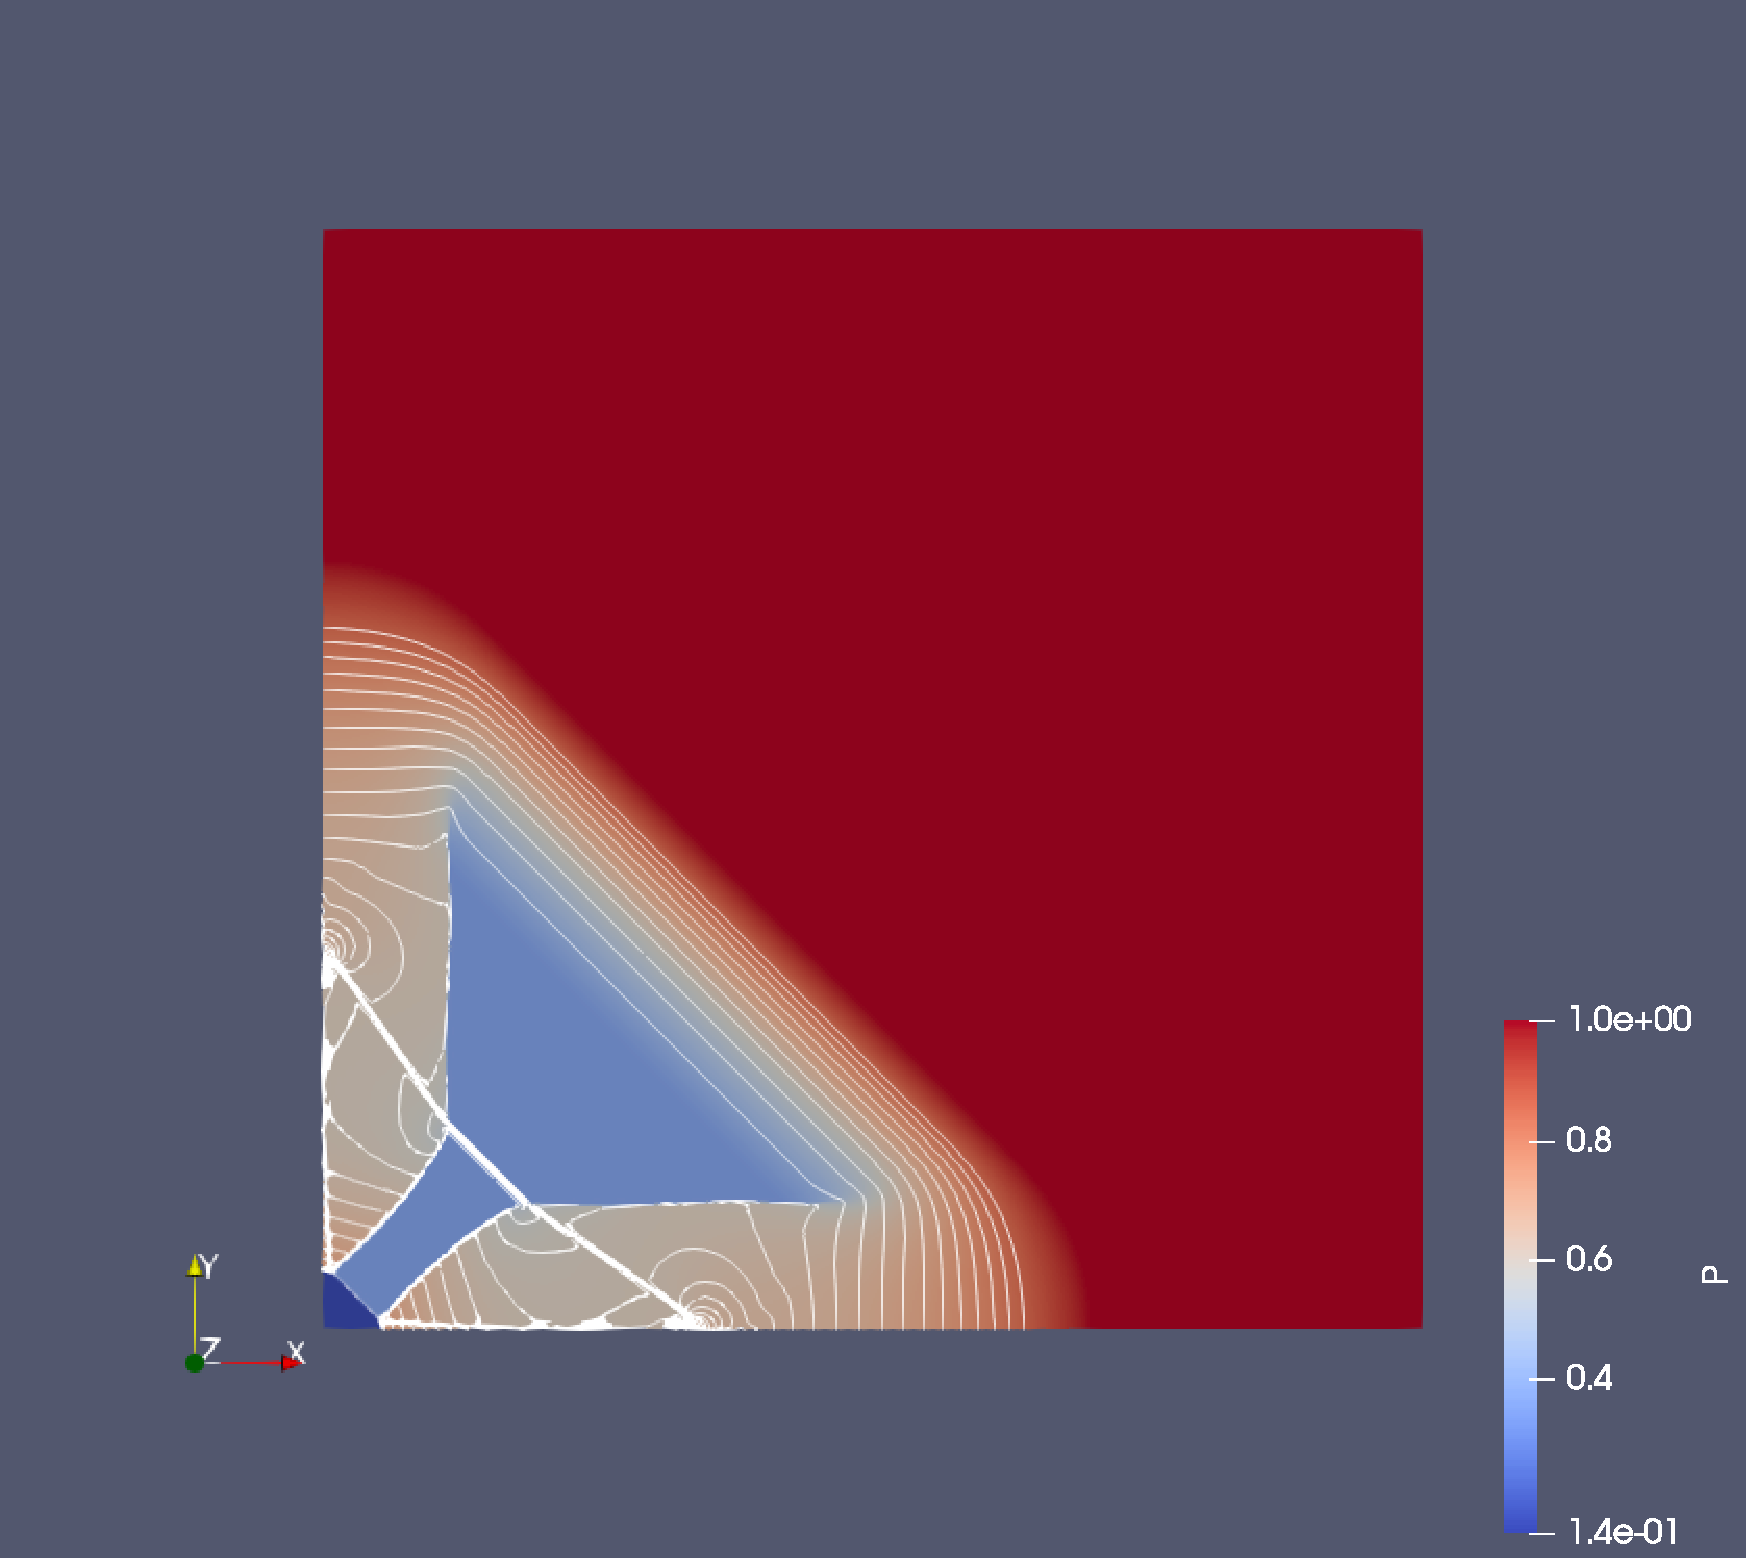
\includegraphics[scale=0.16]{figures/GAH-Hui-400-005.pdf }
\caption{Early time ($t = 0.05$) pressure-density results for the $\beta = 0.$ Hui problem. Density contours show values of $\rho$ in $36$ intervals from $0.125$ to $1.0$.}
  \label{fig:hui-Rot0-005}
\end{subfigure}

\bigskip

\begin{subfigure}[h!]{0.4\linewidth}
\centering
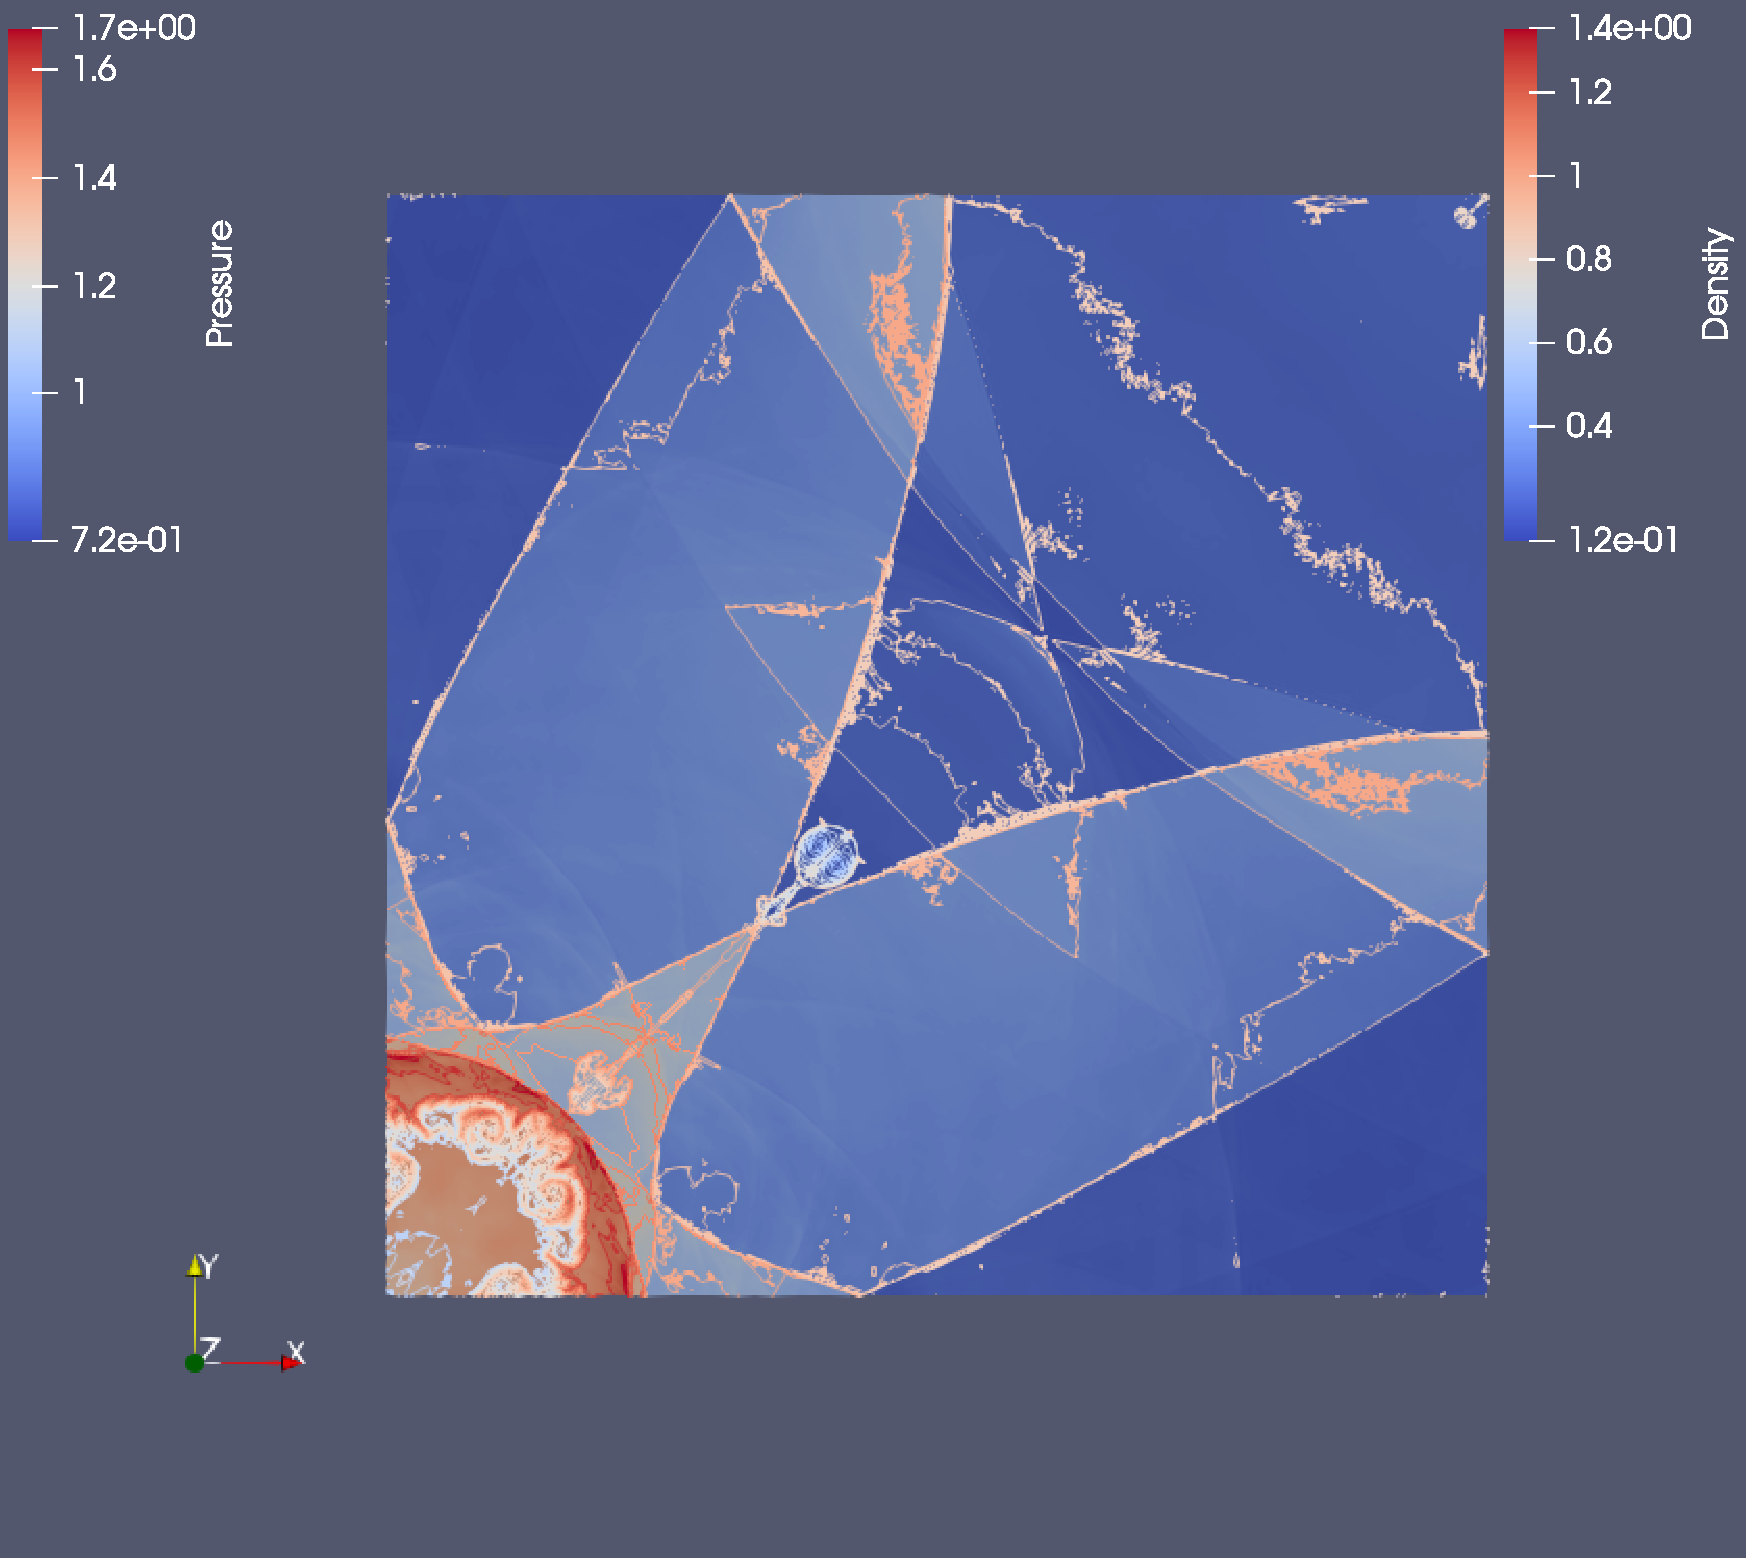
\includegraphics[scale=0.16]{figures/GAH-Hui-400-125.pdf }
\caption{The $t = 1.25$ pressure-density results for the $\beta = 0.$ Hui problem. Density contours show values of $\rho$ in $31$ intervals from $0.35$ to $1.1$.}
  \label{fig:hui-Rot0-125}
\end{subfigure}
\begin{subfigure}[h!]{0.4\linewidth}
\centering
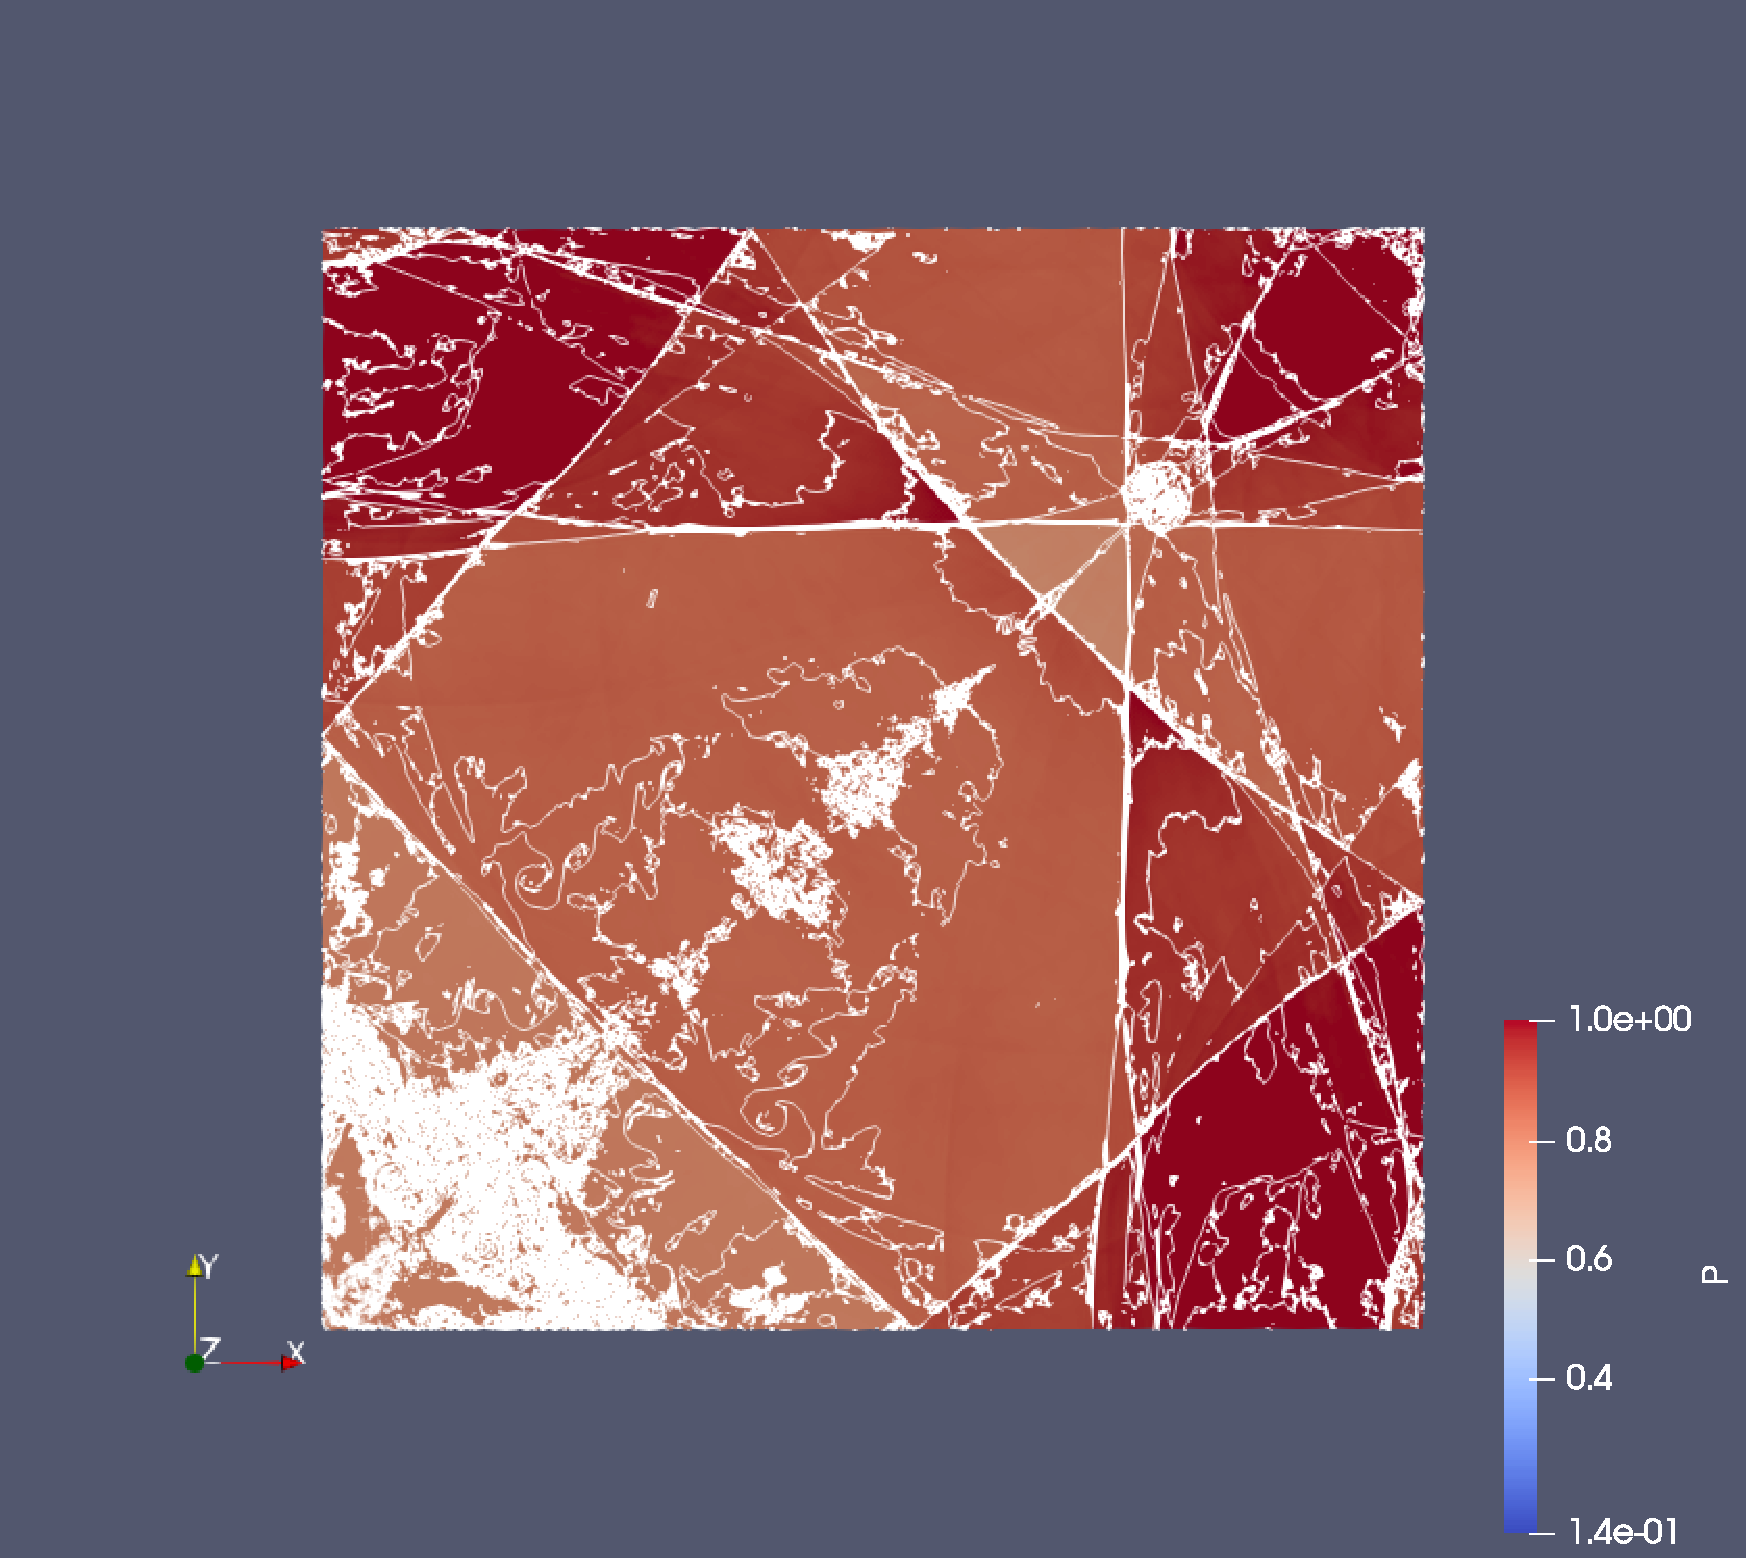
\includegraphics[scale=0.16]{figures/GAH-Hui-400-250.pdf }
\caption{Late time ($t = 2.50$ ) pressure-density results for the $\beta = 0.$ Hui problem. Density contours show values of $\rho$ in $31$ intervals from $0.35$ to $1.1$.}
  \label{fig:hui-Rot0-250}
\end{subfigure}
\caption{The unrotated Hui Problem results.}
\label{fig:hui-Rot0}
\end{figure}

\subsubsection{Rotated mesh}\label{sssec:huiRot}

The results in Figure \ref{fig:hui-Rot} document the case where the box geometry is rotated by $0.4 \ \mathrm{rad}.$ about the $X(3)$ (z coordinate) axis.  The mesh input deck is shown in \ref{ssec:hoprin-hui-Rot} and the Flexi input in \ref{ssec:flexiin-hui-Rot}. The scheme used in the unrotated case (Section \ref{sssec:huiNR})  to assure that the Persson indicator was symmetric about the diagonal line $\overline{42}$ of Figure \ref{fig:HuiGeom} was not used ($\mathrm{IndSym} = 0$).

\begin{figure}[h!]
\centering
\begin{subfigure}[h!]{0.4\linewidth}
\centering
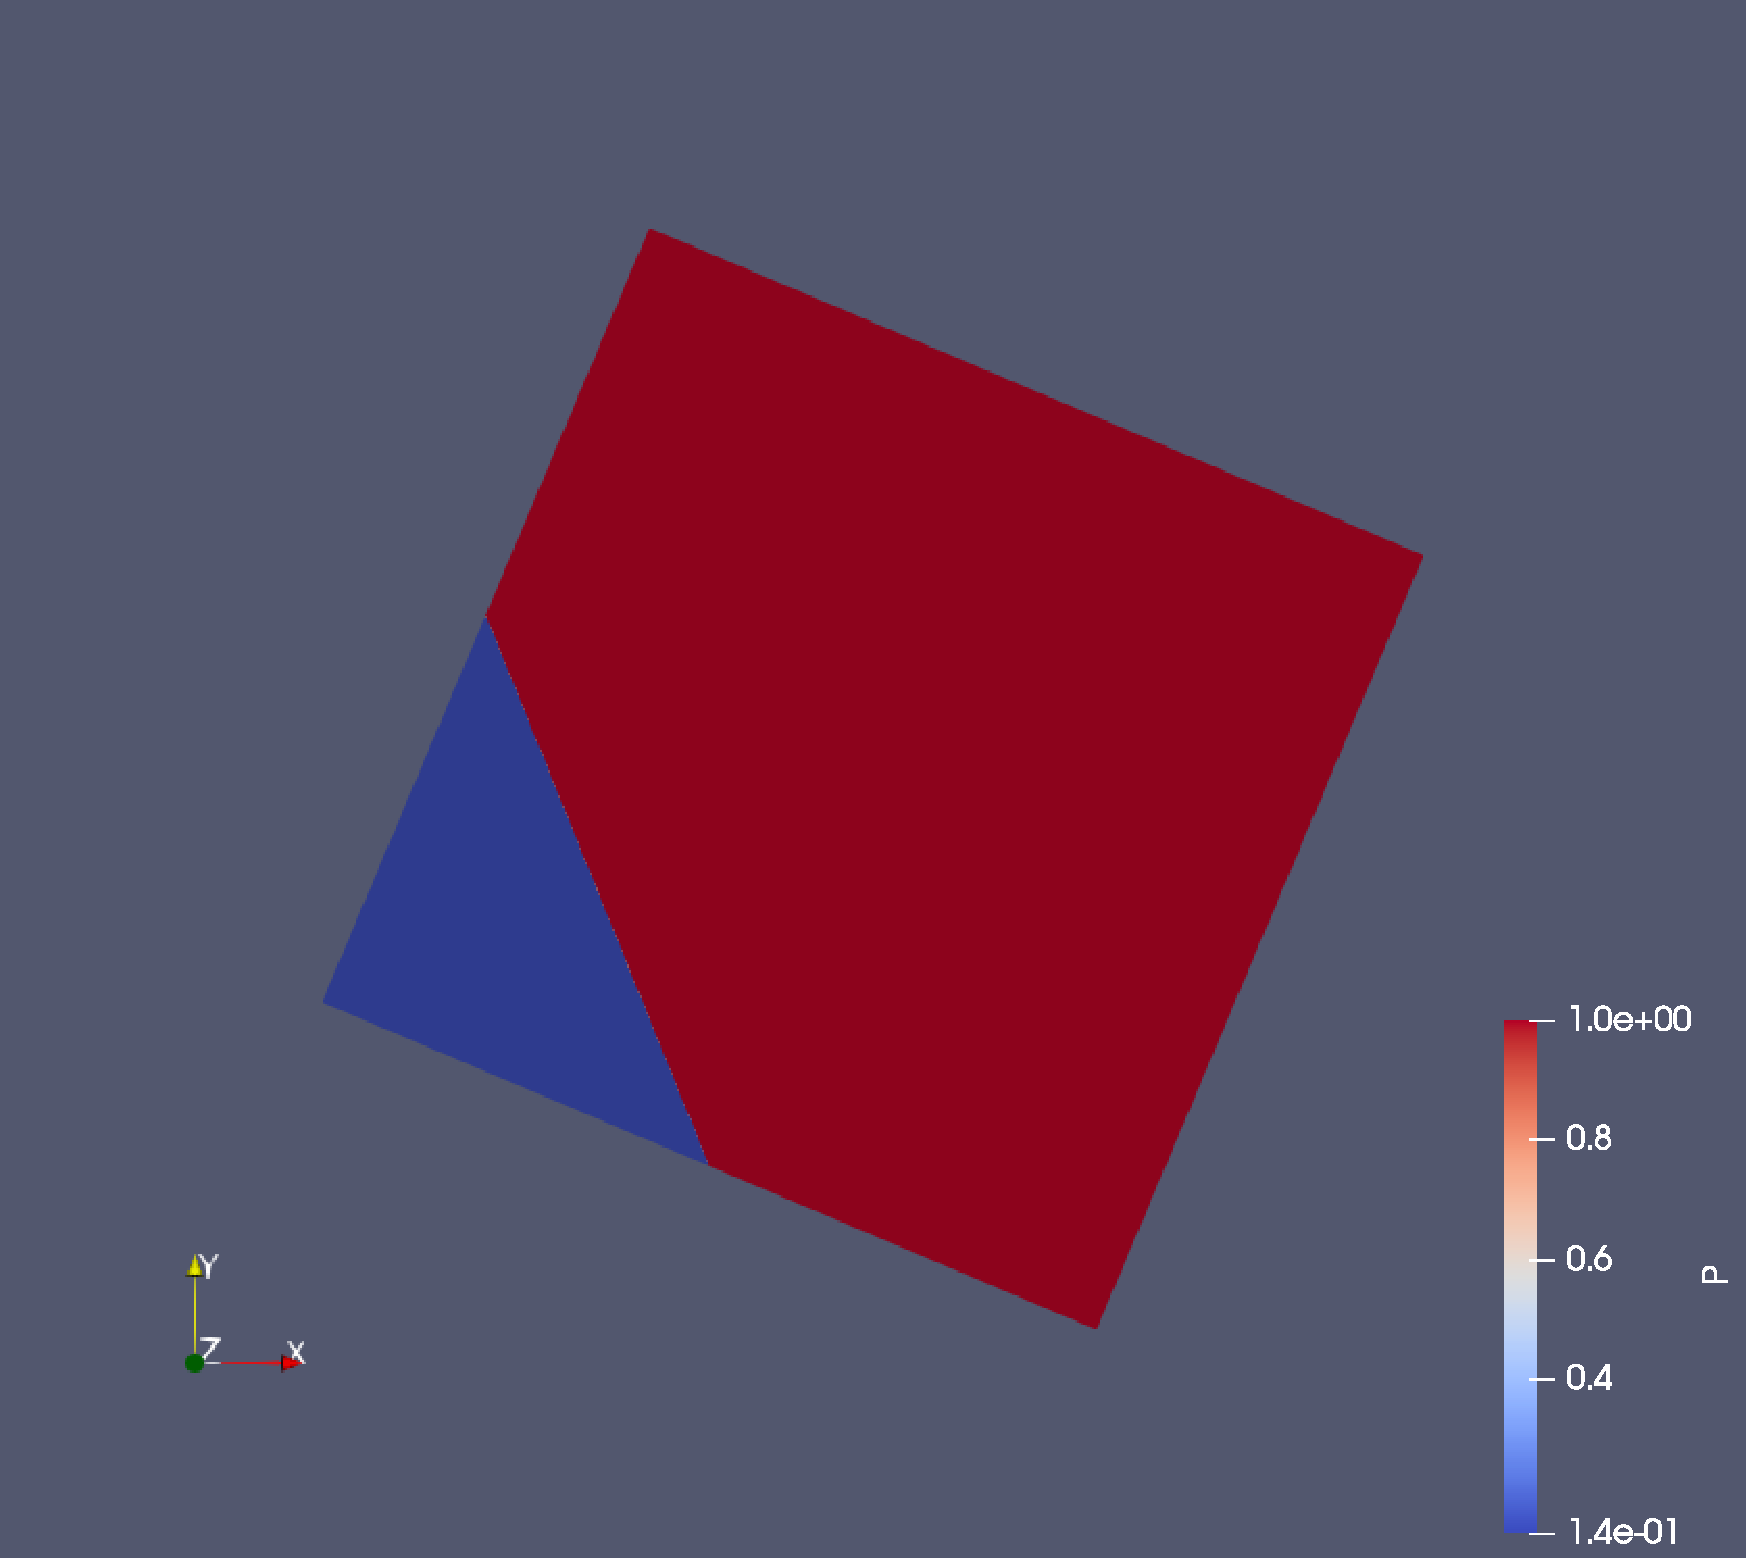
\includegraphics[scale=0.16]{figures/GAH-Hui-400-0000-R.pdf }
\caption{Initial pressure field for the $\beta = 0.4 \ \mathrm{rad.}$ Hui problem.\bigskip \bigskip}
  \label{fig:hui-Rot-0}
\end{subfigure}
\begin{subfigure}[h!]{0.4\linewidth}
\centering
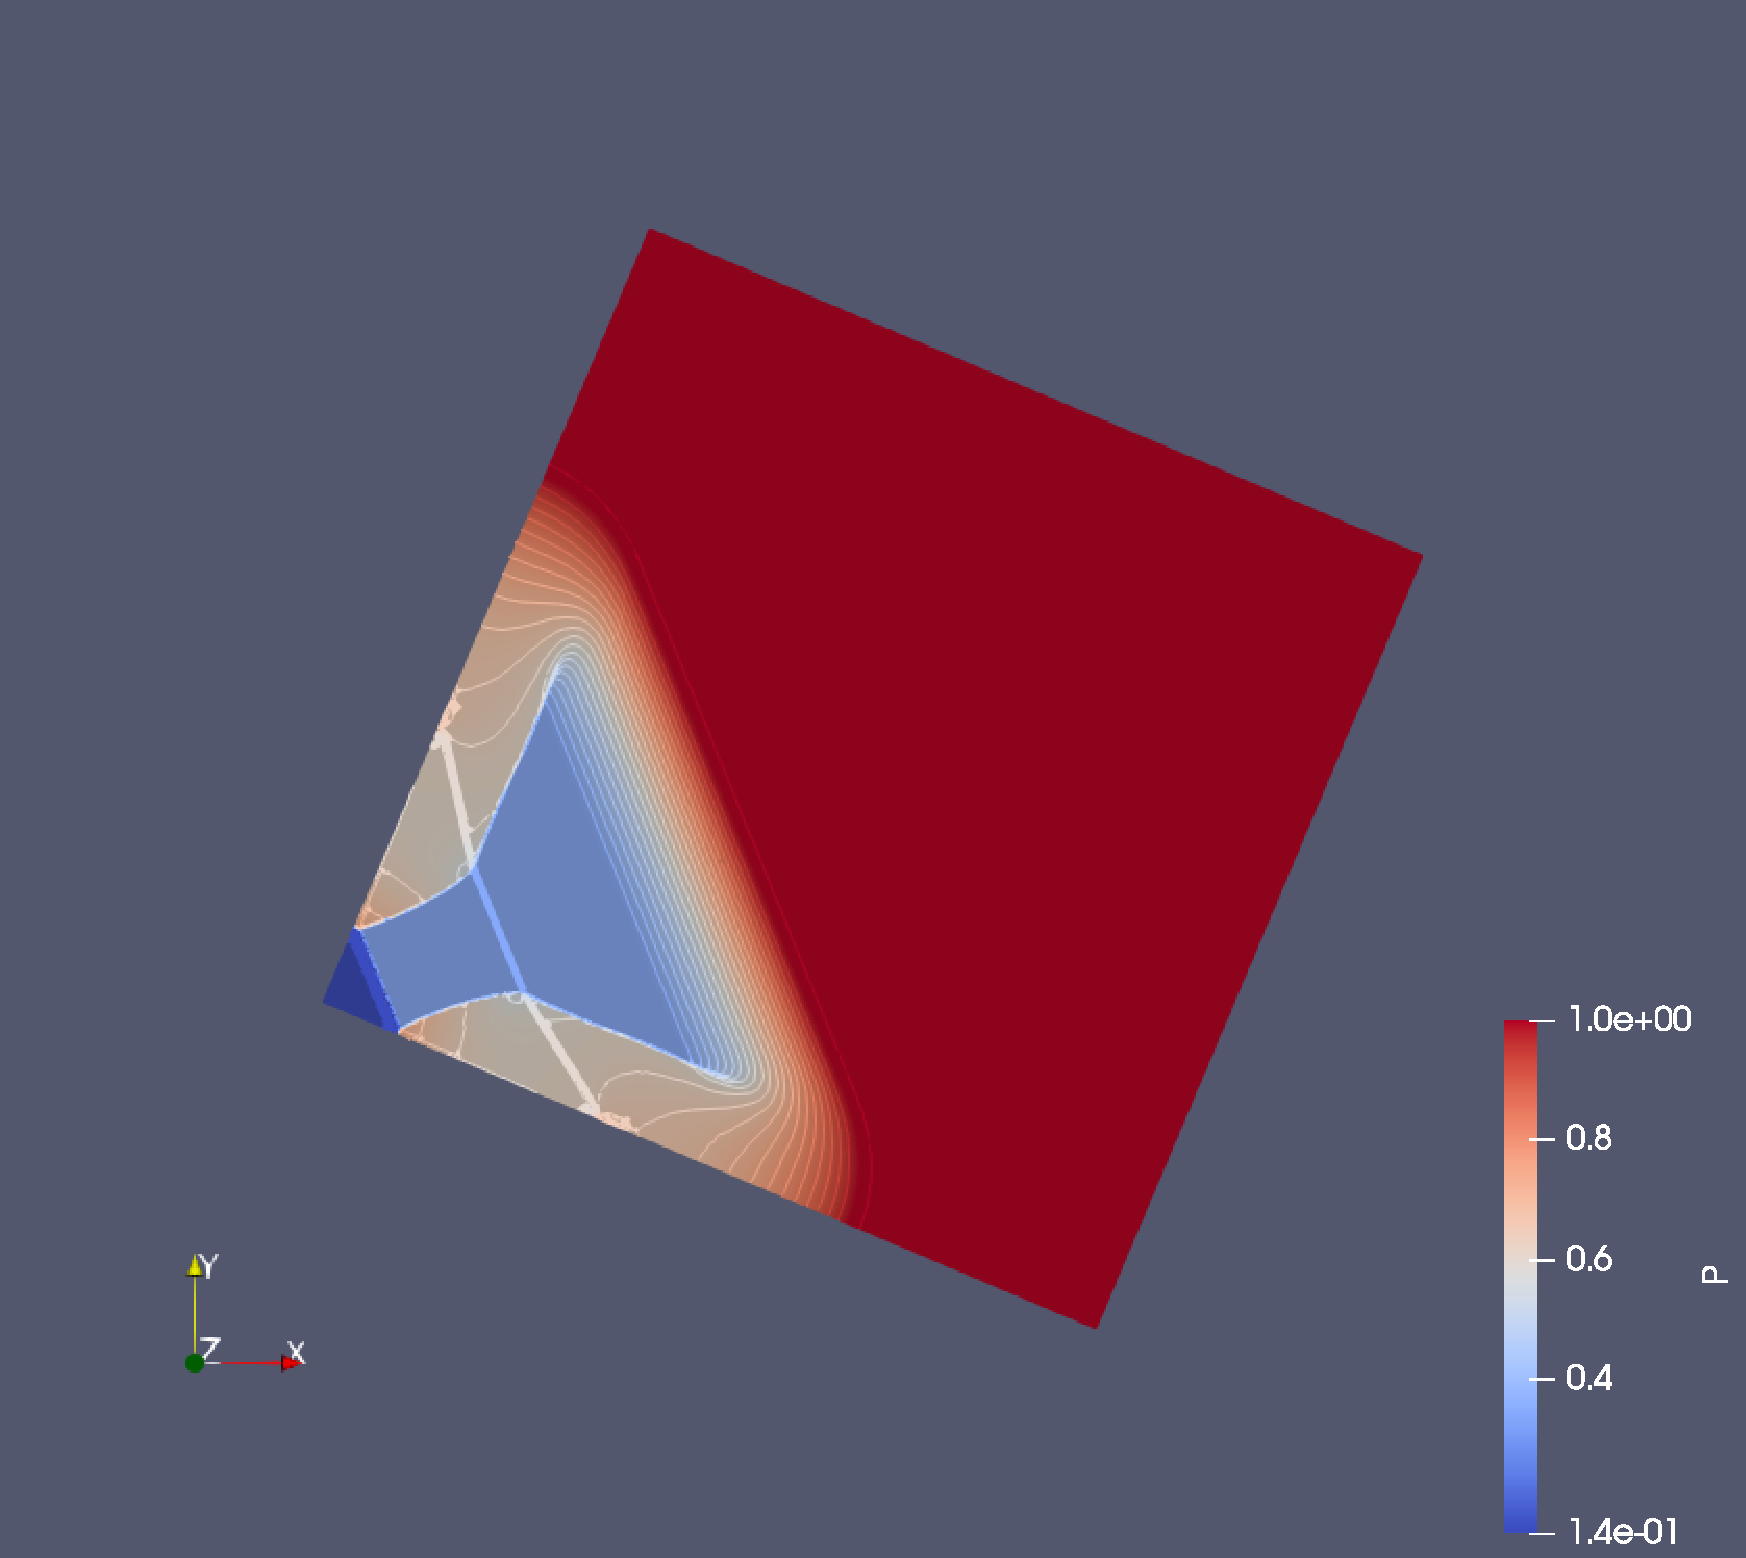
\includegraphics[scale=0.16]{figures/GAH-Hui-400-0045-R.pdf }
\caption{Early time ($t = 0.045$) pressure-density results for the $\beta = 0.4 \ \mathrm{rad.}$ Hui problem. Density contours show values of $\rho$ in $36$ intervals from $0.125$ to $1.0$.}
  \label{fig:hui-Rot-0045}
\end{subfigure}

\bigskip

\begin{subfigure}[h!]{0.4\linewidth}
\centering
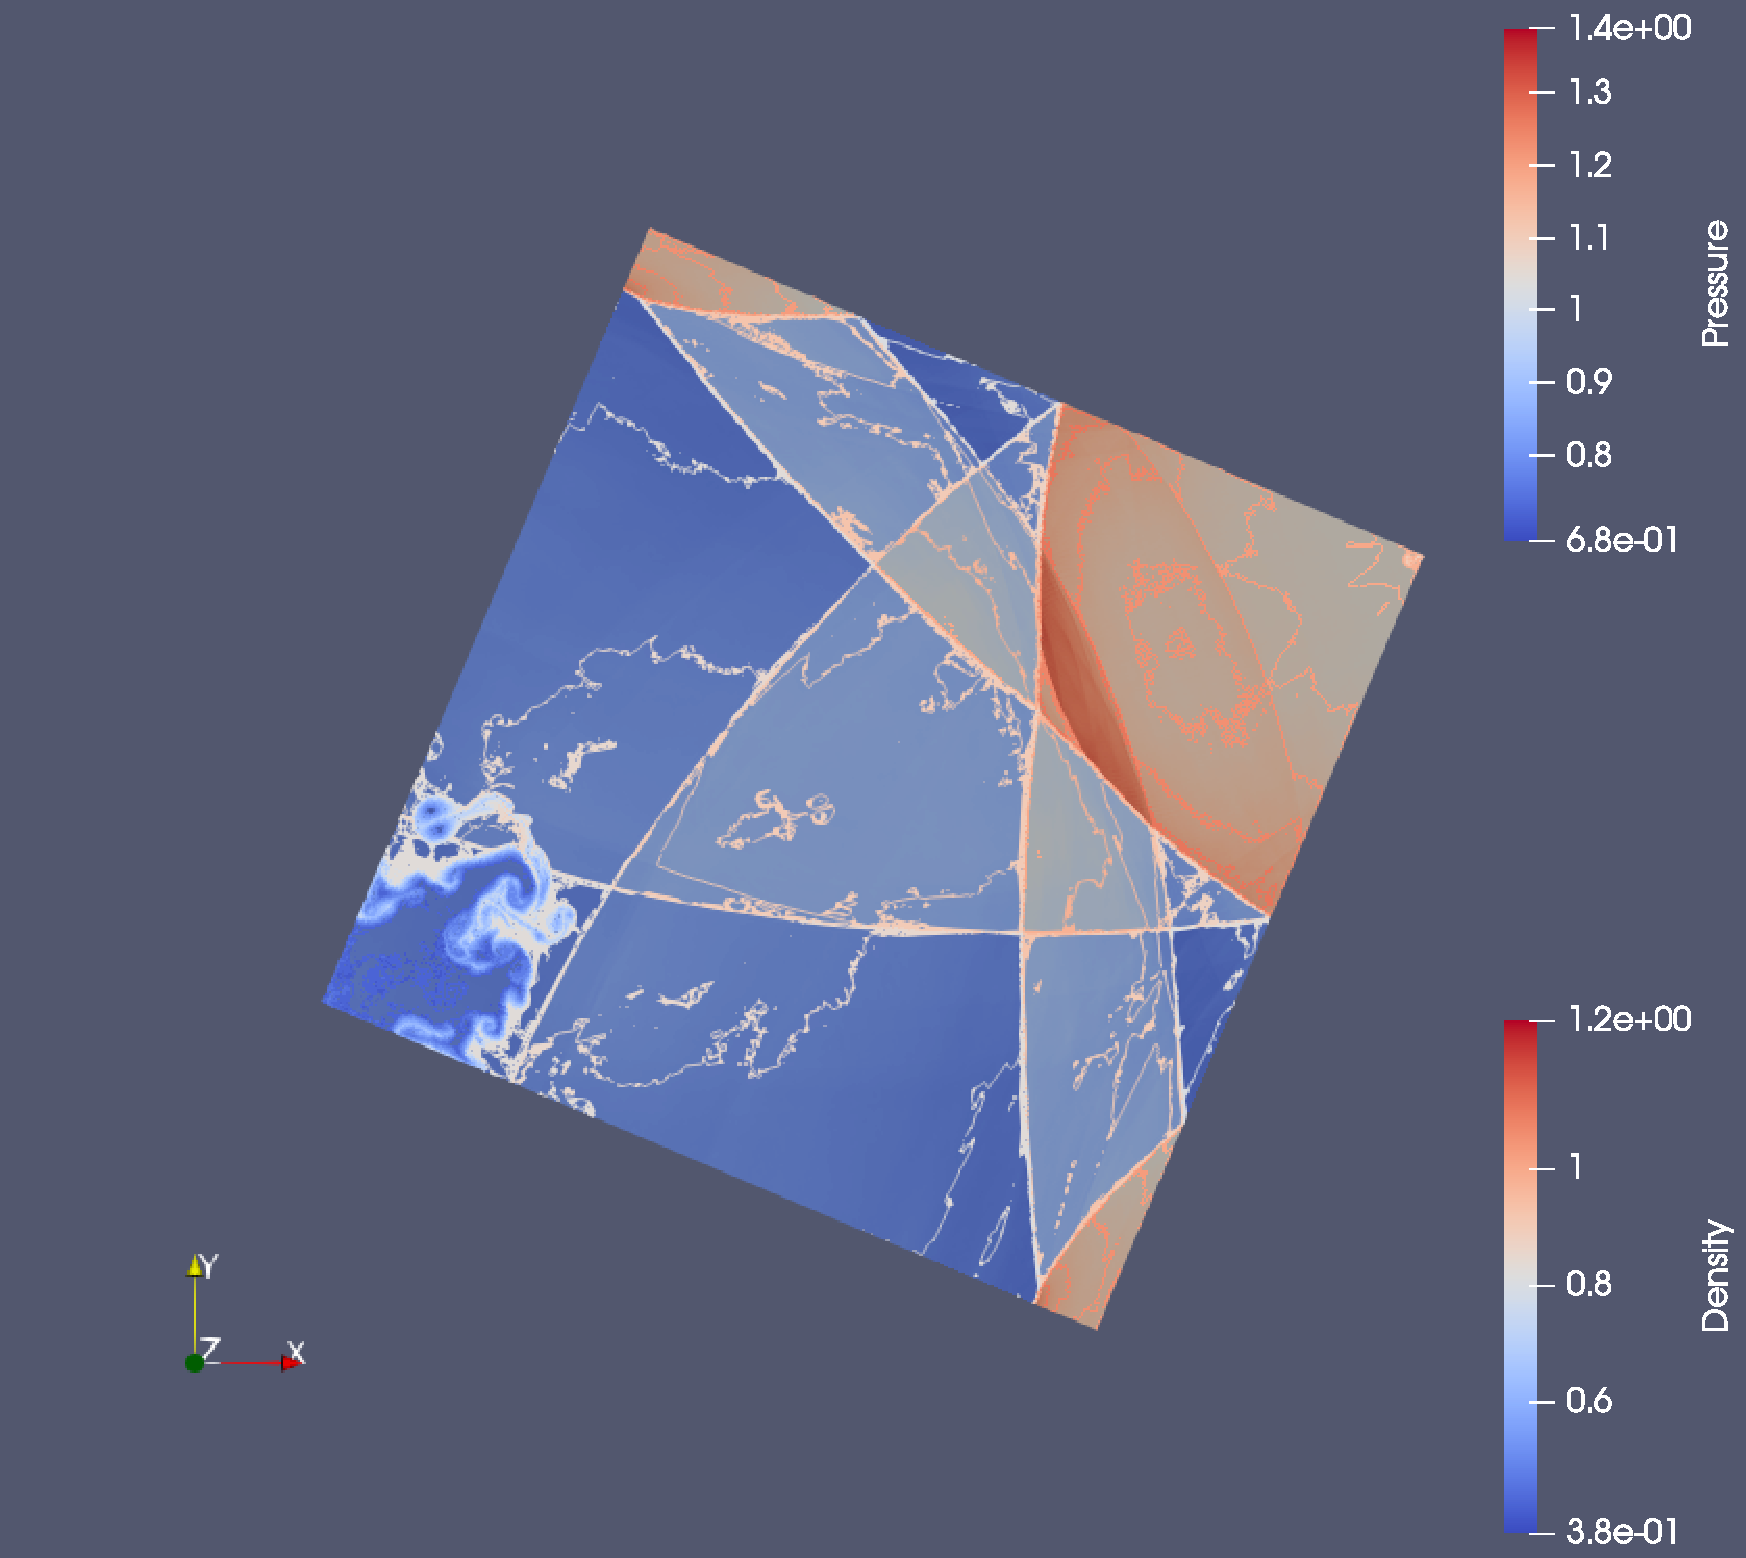
\includegraphics[scale=0.16]{figures/GAH-Hui-400-0100-R.pdf }
\caption{Early time ($t = 0.1$ ) pressure-density results for the $\beta = 0.4 \ \mathrm{rad.}$ Hui problem. Density contours show values of $\rho$ in $31$ intervals from $0.35$ to $1.1$.}
  \label{fig:hui-Rot-250}
\end{subfigure}
\begin{subfigure}[h!]{0.4\linewidth}
\centering
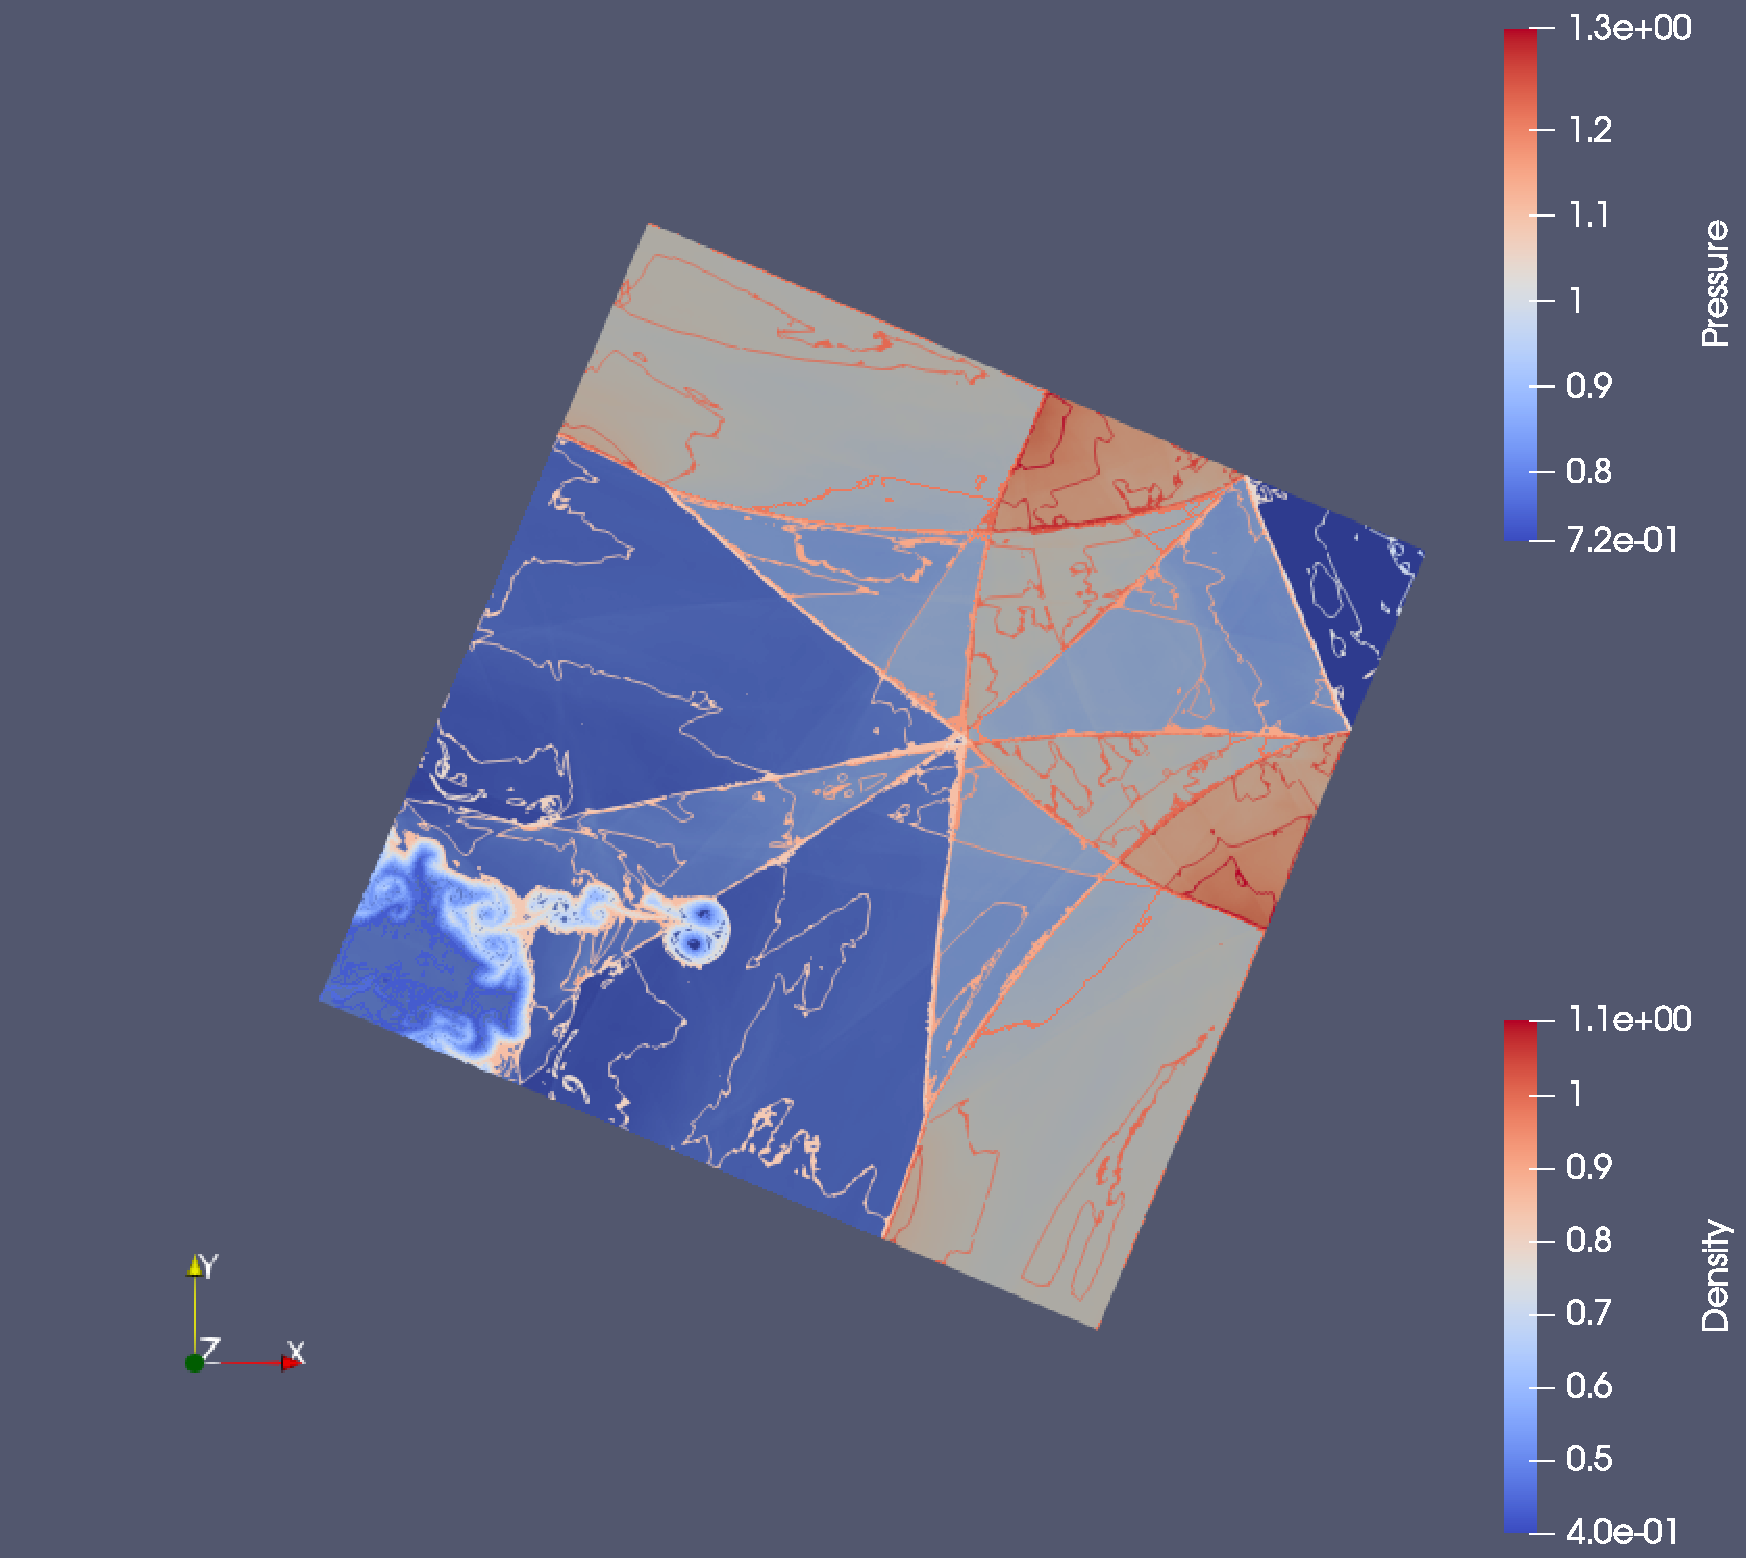
\includegraphics[scale=0.16]{figures/GAH-Hui-400-1500-R.pdf }
\caption{Later time ($t = 1.50$ ) pressure-density results for the $\beta = 0.4 \ \mathrm{rad.}$ Hui problem. Density contours show values of $\rho$ in $31$ intervals from $0.35$ to $1.1$.}
  \label{fig:hui-Rot-1500}
\end{subfigure}

\caption{The rotated Hui Problem results showing asymmetry in the longer time results.  These results did not use the symmetric indicator routine; which gave equally inaccurate results.}
\label{fig:hui-Rot}
\end{figure}

The Hui problem is a very challenging one and Flexi has demonstrated its ability to do well in simulating the problem.  The issues with the rotated mesh results suggests some further review of the code may be necessary.
